% Template for ICIP-2012 paper; to be used with:
%          spconf.sty  - ICASSP/ICIP LaTeX style file, and
%          IEEEbib.bst - IEEE bibliography style file.
% --------------------------------------------------------------------------
\documentclass{article}
\usepackage{spconf,amsmath,graphicx}
\usepackage[tight,footnotesize]{subfigure}

% Example definitions.
% --------------------
\def\x{{\mathbf x}}
\def\L{{\cal L}}

% Title.
% ------
%\title{AUTHOR GUIDELINES FOR ICIP 2012 PROCEEDINGS MANUSCRIPTS}
\title{Efficient Real-time Similarity Detection\\for Video Caching and Streaming}
%
% Single address.
% ---------------
%\name{Author(s) Name(s)\thanks{Thanks to XYZ agency for funding.}}
\name{Victor K.Y. Wu and Constantine Polychronopoulos}
%\address{Author Affiliation(s)}
\address{Bytemobile, Inc.}
%
% For example:
% ------------
%\address{School\\
%	Department\\
%	Address}
%
% Two addresses (uncomment and modify for two-address case).
% ----------------------------------------------------------
%\twoauthors
%  {A. Author-one, B. Author-two\sthanks{Thanks to XYZ agency for funding.}}
%{Victor K.Y. Wu}
%{wu.victor@gmail.com}
%	{School A-B\\
%	Department A-B\\
%	Address A-B}
%  {C. Author-three, D. Author-four\sthanks{The fourth author performed the work
%	while at ...}}
%{Constantine Polychronopoulos}
%{Bytemobile, Inc.\\constantine@bytemobile.com}
%	{School C-D\\
%	Department C-D\\
%	Address C-D}
%
\begin{document}
\ninept
%
\maketitle
%
\begin{abstract}
We present an enterprise-level Internet video cache and streaming system that generalizes ``cache hits" to videos that are at least similar, human perception-wise. When a user requests a video not in our cache, our system starts streaming the video from the Internet, and forwards it to the user. We efficiently extract feature vectors from the incoming byte stream, comparing them to feature vectors of cached videos, all in real time. After a short period, we may decide that we have a similar video (but that is not byte-wise identical). We then stop the Internet-side download, and continue streaming to the user using the similar video instead, saving valuable resources. Our system makes similarity decisions with rates of incorrectness approaching zero, after only $30$ seconds of Internet-side streaming.
%The abstract should appear at the top of the left-hand column of text, about
%0.5 inch (12 mm) below the title area and no more than 3.125 inches (80 mm) in
%length.  Leave a 0.5 inch (12 mm) space between the end of the abstract and the
%beginning of the main text.  The abstract should contain about 100 to 150
%words, and should be identical to the abstract text submitted electronically
%along with the paper cover sheet.  All manuscripts must be in English, printed
%in black ink.
\end{abstract}
%
\begin{keywords}
Video similarity detection, video caching, video streaming
%One, two, three, four, five
\end{keywords}
%

\section{Introduction}
Consider an enterprise-level video cache system situated between Internet users and content providers, as shown in Fig. \ref{figure:Video Caching System}. Our ideas are conceptual in nature. But one can imagine the caching system to be implemented within a variety of networks, such as an Internet service provider (ISP), a private intranet, or a mobile wireless network. Previous work has already touched on cache hits in the traditional sense, where a streaming video request is served from the cache if there is a byte-wise identical copy already stored in the cache. In this work, we generalize the notion of cache hits to detecting and serving \emph{similar} videos in \emph{real time}. That is, suppose a user in Fig. \ref{figure:Video Caching System} requests a video. Our cache first checks if an identical copy is already stored, as usual. If not, our cache starts downloading the video from the content provider (storing it in memory), while at the same time begins streaming it to the user. Our cache \emph{efficiently} extracts information \emph{directly} from the incoming video byte stream in real time, forming an increasingly large video signature. We then compare this signature with pre-calculated signatures of the cached videos in real time. After a short period, we may decide that there is a similar video in the cache (human perception-wise), that matches the incoming video. We then stop downloading the incoming video, and use the cached similar video instead to continue streaming to the user. If we decide that there are no similar videos, everything proceeds as usual, like a traditional video cache.

In this work, our main contribution is thus an efficient real-time similarity detection scheme that makes our caching system possible. Reducing storage size is an obvious benefit for traditional caches. Our system further amplifies this since many Internet videos are similar, but not recognized as such by current systems, since similar videos are entirely different, byte-wise. In particular, as videos are downloaded by users, processed, and re-uploaded to the Internet, they are changed slightly, but their subsequent similarities are not exploited in caching systems. These changes are due to different codecs and container formats, different resolutions, different filtering effects such as sharpening or blurring, watermarking, metadata additions, etc. Often, the modifications are slight, and barely noticeable to users, who may not mind being served similar videos, especially if the overall experience is better (no video jitter, for example). Note that in this work, we do not objectively define what similarity is, human perception-wise. Rather, we provide a set of examples that \emph{should} be humanly similar, and evaluate our algorithmic definition of similarity against these examples. Furthermore, there may be other issues, in particular legal arguments, that factor in a cache serving non-byte-identical videos. It is beyond the scope of this work to consider these ideas. But we believe they will solve themselves in time, given the motivating benefits of our system.

Since we envision our cache system to operate in an enteprise environment, supporting thousands of simultaneous users, another benefit beyond storage size reduction is processing load savings. If a similar video is found, the Internet side connection of Fig. \ref{figure:Video Caching System} is stopped. This signficantly reduces processing load, especially if the cache was doing intermediate processing (e.g. video transcoding on the fly to fit the user) prior to connection stoppage. That is, the cache can just serve a pre-processed version (appropriate for the user) of the similar video that is already stored in the cache.

Finally, recognizing video similarity in itself has many benefits, including enhancing the user experience, as well as providing user analytics (e.g. video consumption behavior) to the entity operating the video cache.

\begin{figure}
\centering
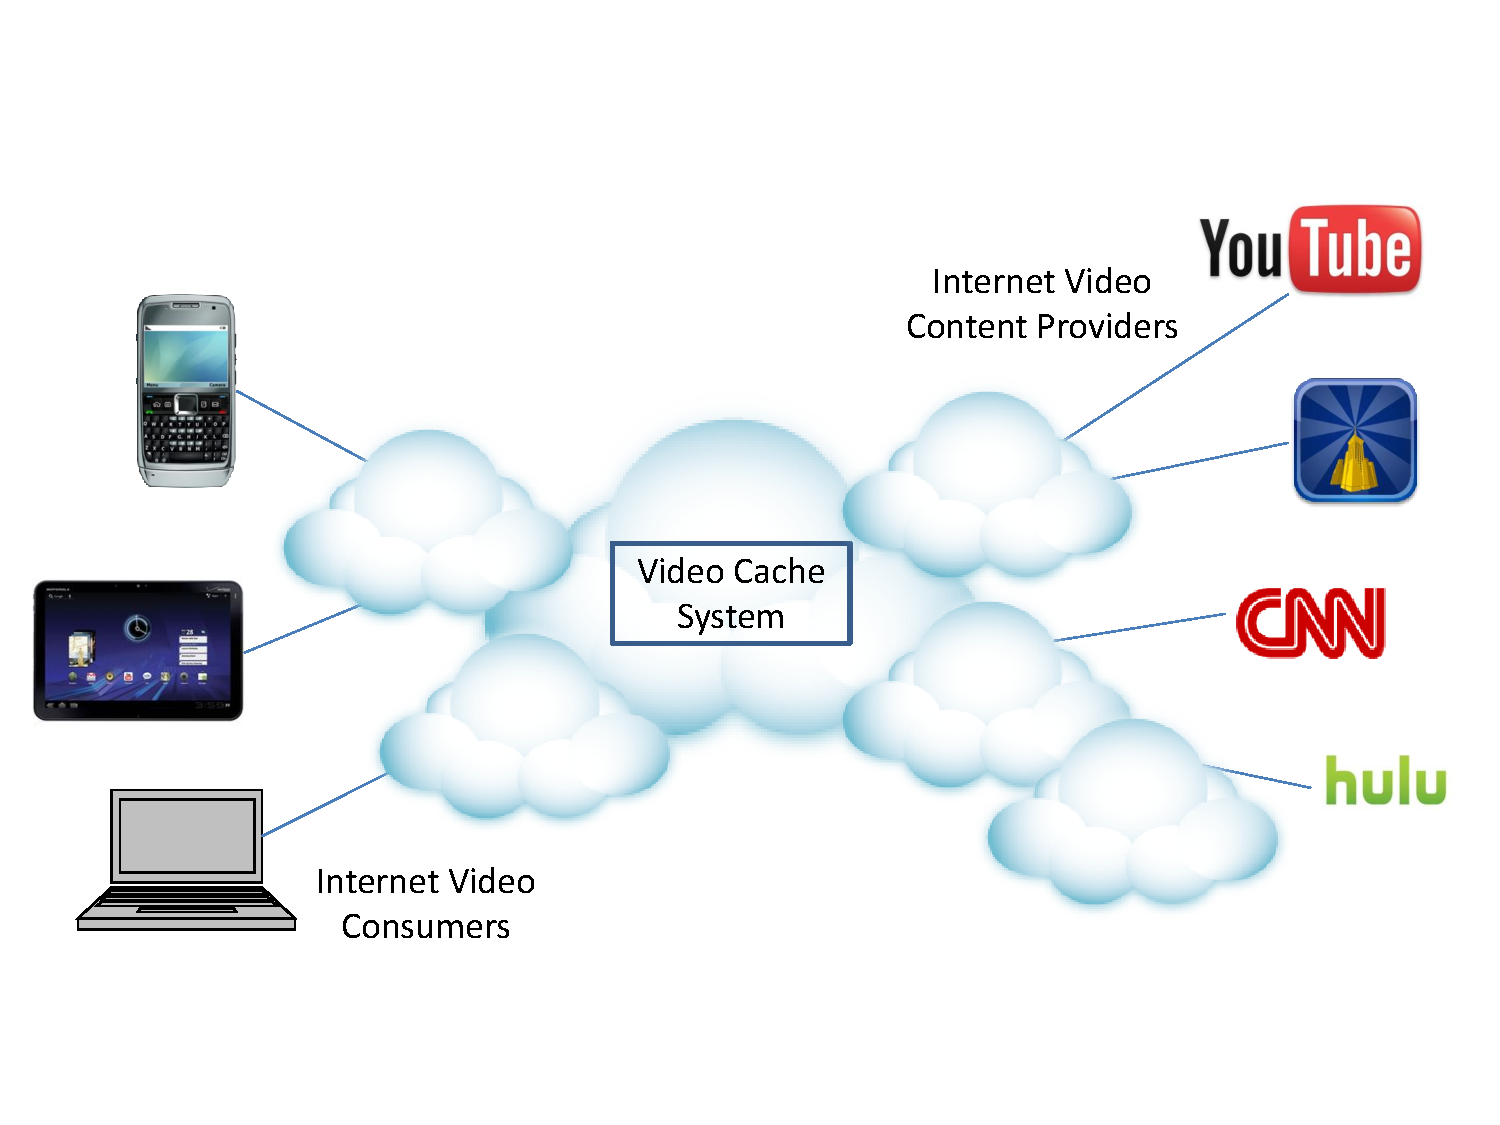
\includegraphics[height=1.3in, viewport=0 75 700 445, clip]{video_cache.pdf}
\caption{Video Caching System}
\label{figure:Video Caching System}
\end{figure}

\subsection{Background Literature}
Previous work in video caching increases the cache dimensionality using a variety of methods. The authors in \cite{Songqing Chen}, \cite{Wei Tu}, \cite{Dohy Hong} divide individual videos into mutliple time chunks. Small chunks are cached, instead of large individual video objects. The authors in \cite{Yago Sanchez} cache coding layers of a video separately, serving only as many layers as needed to recover a requested quality level. The authors in \cite{Jing Li} cache videos over a set of distributed servers. Video requests are re-directed to the server containing the stored video. The authors in \cite{Byoung-Jip Kim} store different transcoded versions of the same video in different proxies. 

Overall, these methods improve cache efficiency by granularizing space, time, and code dimensions. Our work furthers this generalization by leveraging the video content itself by granularizing the human perception of video.

Previous work in video de-duplication \cite{Chuanyi Liu}, \cite{Atul Katiyar} and video similarity detection \cite{Sen-ching S. Cheung}, \cite{Xian-Sheng Hua} both employ video signatures. A video signature is a compact representation of a video, in a necessarily lower dimesional space, compared to the video itself. In de-duplication (where the application is primarily increasing storage efficiency), the video signature should be as unique as possible. It is thus like a hash. In video similarity detection, the video signature should additionally be robust, so that small changes in the video should not significantly change the signature. In this sense, it is not like a hash. These difficult (and often opposing requirements) have resulted in computationally heavy siganture generation algorithms, which we therefore cannot use, since they oppose our goals of light computation and real-time performance.

\subsection{Paper Outline}
In Section \ref{section:Real-time Video Similarity Detection System}, we outline our real-time video similarity detection system. We provide experiments in Section \ref{section:Experiments}. In Section \ref{section:Real-world Implementation Considerations}, we consider issues arising from a real-world implementation. Finally, we conclude in Section \ref{section:Conclusion}.

\section{Real-time Video Similarity Detection System}
\label{section:Real-time Video Similarity Detection System}

\subsection{System Model}
Our video cache system is situated between Internet users and content providers, as shown in Fig. \ref{figure:Video Caching System}. Initially, there are $N$ stored videos, each with a different time length, $t_i$ seconds, in general, where $i \in \{0, \ldots, N-1\}$. Let $T$ seconds be a time epoch that is smaller than $\min_i t_i$, but larger than the typical period between consecutive I-frames (intra-frames) in a video. We divide each video into consecutive $T$ second time chunks, so that the $i^{th}$ video has $\lceil \frac{t_i}{T} \rceil$ chunks. For example, if video $0$ is $t_0 = 62$ seconds long and $T = 3$ seconds, then its $21$ associated chunks are $\{0-3, 3-6, \ldots, 57-60, 60-62\}$ seconds. For each video, we form a feature vector representing each chunk. The ordered collection of all feature vectors $\{f_k\}$ of the $i^{th}$ video forms its video signature, $s^{(i)}$. Continuing from our previous example, video $0$ has signature $s^{(0)} = \left( f^{(0)}_0, f^{(0)}_1, \ldots, f^{(0)}_{20} \right)$. The video signatures are also stored in the cache.

To form the feature vector belonging to a chunk, we first consider only the I-frames within that chunk. Then, for each of those I-frames, we extract a fraction of the DCT (discrete cosine transform) coefficients representing the image, at fixed locations. Suppose we take $n$ DCT coefficients for each I-frame, forming a length $n$ vector. We then average over all the vectors representing I-frames within that chunk. The resulting length $n$ vector is thus our feature vector $f$. In the unlikely case that the chunk has no I-frames, just let its feature vector be the same as the previous chunk's. If the chunk has no I-frames and is the first chunk, then just let its feature vector be the zero vector.

\subsection{Similarity Definition}
\label{subsection:Similarity Definition}
We define an algorithmic notion of similarity. It is our goal that this closely matches our human perception of similarity, which we do not define here. But we do evaluate our system against reasonable ``human cases of similarity" in the experiment sections below. If two videos have different number of chunks, they are defined to be dissimilar. If two videos have the same number of chunks, $C$, we define similarity up to the $c^{th}$ chunk, where $c \in \{0, \ldots, C-1\}$, with respect to threshold $e_{thres}$. The cumulative error between two videos up to the $c^{th}$ chunk is the sum of the first $c+1$ L2 vector norms of feature vector differences. That is, the cumulative error between videos $i$ and $j$ is:
$e^{(c)}_{i,j} = \sum_{k=0}^c  \left|\left| f^{(i)}_k - f^{(j)}_k \right|\right|_2$. We say that videos $i$ and $j$ are similar if $e^{(c)}_{i,j} \leq e_{thres}$, for $c$ and $e_{thres}$ chosen in advance. Otherwise, they are dissimilar.

\subsection{Real-time Similarity Detection Algorithm}
\label{subsection:Real-time Similarity Detection Algorithm}
Similarity detection occurs in two stages as a video is being downloaded from the Internet.  First, we determine the incoming video's length (and thus, the number of chunks it will be divided into) by reading the metadata readily available in most video containers and codecs early in the byte stream. We then eliminate many candidates from our video cache based on the same number of chunks criterion. (We can use other metadata as well for further filtering. We discuss this later.) In stage two, we form feature vectors from the incoming video by extracting DCT coefficients directly from its byte stream. We then compare these feature vectors with the feature vectors of existing videos in the cache. All this is performed in real time. After $c$ chunks have been formed and compared, we determine if there is (are) similar video(s). If yes, we take the candidate with the smallest cumulative error with respect to the incoming video. Otherwise, we decide that the incoming video is dissimilar to all the existing ones in the cache. It is a new video.

\begin{figure*}
\centering
\subfigure[Original Video]		   {
\includegraphics[width= 1.35in, viewport=0 5 650 400, clip]{original} \label{subfigure:original}}
\subfigure[Sharpened Video]     {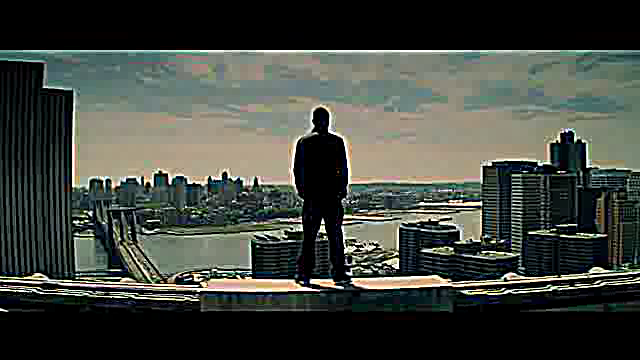
\includegraphics[width= 1.35in, viewport=0 5 650 400, clip]{sharpened}\label{subfigure:sharpened}} 
\subfigure[Blurred Video]       {
\includegraphics[width= 1.35in, viewport=0 5 650 400, clip]{blurred}  \label{subfigure:blurred}}
\subfigure[Logo in Top Left]    {
\includegraphics[width= 1.35in, viewport=0 5 650 400, clip]{logo_tl}  \label{subfigure:logo_tl}}
\subfigure[Logo in Bottom Right]{
\includegraphics[width= 1.35in, viewport=0 5 650 400, clip]{logo_br}  \label{subfigure:logo_br}}
\caption{Filtering and Watermarking (logo is $\frac{1}{4}$ width)}
\label{figure:Filtering and Watermarking}
\end{figure*}

\section{Experiments}
\label{section:Experiments}
We consider how effective our algorithm is at detecting three notions of human perception-wise similarity. Also, we disregard stage one of the detection algorithm. (This is future work.) Rather, we focus on the actual similarity detection using feature vector comparisons. For the videos in our experiment, we consider only the first $60$ seconds of each, and take $T = 3$ seconds. Therefore, there are $C = 20$ chunks for all videos. For I-frames, we consider $48$ preset ``areas" of only the luminance image. The areas are normalized to a reference image resolution (allowing our algorithm to be robust to different resolutions). The area locations are biased toward the center of the image, to avoid artifacts sometimes near image borders. The reference image resolution is $96 \times 54$ blocks, where one block is $8 \times 8$ pixels. The $48$ preset areas of the reference image resolution are actually blocks, identified by $8$ column block indices and $6$ row block indices. These zero-based indices are $\{16, 24, 32, 40, 48, 56, 64, 72\}$ and $\{9, 15, 21, 27, 33, 39\}$, respectively. For each area, we consider the DCT coefficent blocks in that vicinity, and spatially average them into one representative block. We then take the first four DCT coefficients of that block (the four lowest frequency coefficients) of that averaged block. Therefore, $n = 4 \times 48 = 192$.

\subsection{Experiment 1: Different Resolutions}
On December 20, 2011, we visited YouTube, and considered the $20$ most viewed videos of all time, that are each within $1$ and $5$ minutes. In particular, for each of these videos, we considered only the following three resolutions: $360$p, $480$p, and $720$p. Only $360$p was available for all $20$ videos. The other two resolutions were not available for every video. But we downloaded as many of these as were available. (Note also that the downloaded videos are not actually exactly at these resolutions. The actual pixel width and pixel height of the downloaded videos are mostly close to these three standards.) We then transcoded all the videos so that everything was encoded using the Sorenson flavor \cite{web:SWF} of the H.263 codec \cite{web:H.263} using FFmpeg \cite{web:FFmpeg}. We used this relatively old codec since it was much easier to extract DCT coefficients when parsing the video byte stream. In future work, we consider more modern codecs. The $20$ videos (disregarding their different resolutions) are all visually dissimilar (human perception-wise).

For each $360$p video, it is defined to have up to two similar (human perception-wise) videos, namely its $480$p and $720$p versions (if they exist). All other videos are dissimilar. For each $360$p video, we calculate its cumulative error with respect to all videos, for all $c \in \{0, \ldots, 19\}$. We aggregate all cumulative error values to form two groups of empirical cumulative distribution functions (CDFs). $E^{(c)}_{sim}$ is the empirical random variable representing the cumulative error up to the $c^{th}$ chunk between any two similar videos. $E^{(c)}_{dis}$ is the random variable representing the dissimilar counterpart. The CDFs of these two random variables are shown in Fig. \ref{subfigure:CDFs:Different Resolutions}. We see that $E^{(c)}_{sim}$ is concentrated at small values, as expected. $E^{(c)}_{dis}$ is spread over more values. As $c$ increases, the cumulative error increases, and therefore $E^{(c)}_{dis}$ is generally larger. Most importantly, the two CDFs have significant separation, indicating that it should be easy to distinguish similar and dissimilar videos, which we consider next.

We consider the rates of incorrectness of our similarity detection decisions. That is, after $c$ chunks are compared between two videos, we decide similarity or dissimilarity based on a threshold, as explained in Section \ref{subsection:Similarity Definition}. We compare this decision against the ``true" human notion of similarity. A false negative is when our algorithm decides that two videos are dissimilar, when they are humanly similar. The false negative rate (fnr) is thus the number of false negatives divided by the total number of compared dissimilar videos. Similarly, a false positive is when our algorithm decides that two videos are similar, when they are humanly dissimilar. The false postive rate (fpr) is thus the number of false positives, divided by the total number of compared similar videos. We plot the fnrs and fprs for different values of $e_{thres}$ in Fig. \ref{subfigure:Rates:Different Resolutions}. As expected, fnr drops as $e_{thres}$ increases, eventually going to zero. Conversely, fpr starts at zero for low $e_{thres}$, and rises to one for high $e_{thres}$. We see that both fnr and fpr are minimized and (approach zero) \emph{together}. That is, we do not need to trade off one for the other. In particular, the smallest $c$ that makes both fnr and fpr equal to zero is $c = 9$, if we choose $e_{thres} = 2.3625$. This means after $10 \times 3 = 30$ seconds, we can make a perfect similarity decision, given this data set.
\begin{figure*}
\centering

\subfigure[CDFs: Different Resolutions]                     {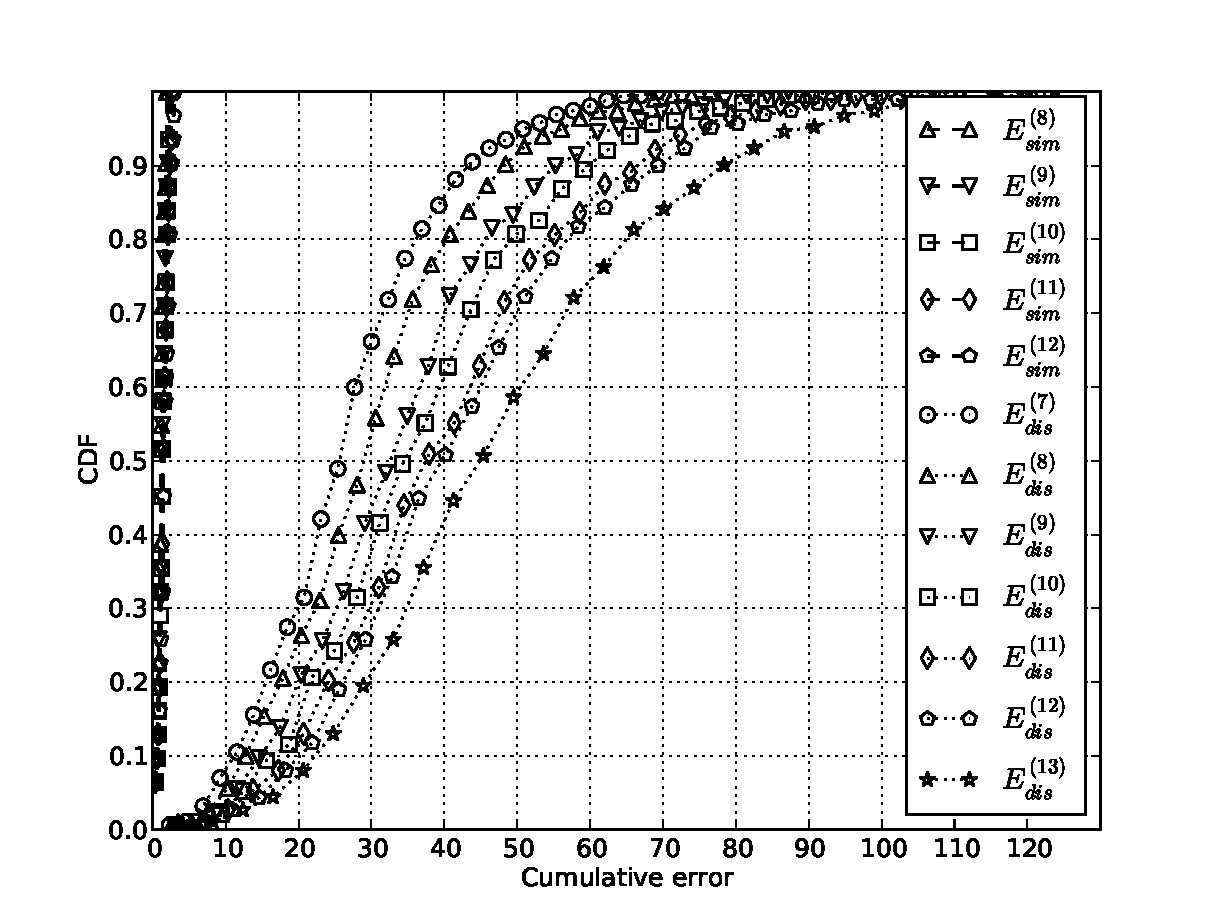
\includegraphics[width=1.1in, height=1in, viewport=0 15 530 400, clip]{resolutions_cdfs}
\label{subfigure:CDFs:Different Resolutions}}
\subfigure[CDFs: Watermarking (logo is $\frac{1}{4}$ width)]{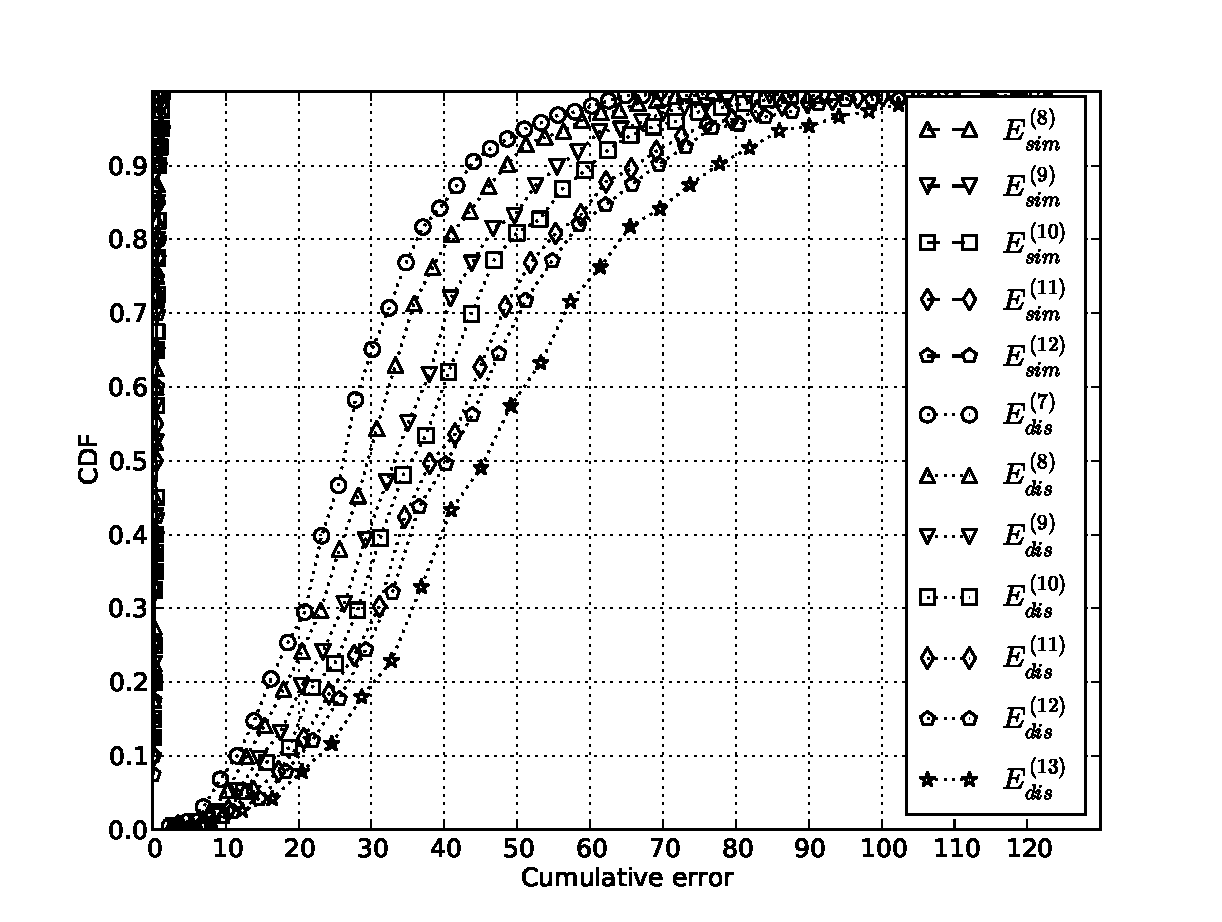
\includegraphics[width=1.1in, height=1in, viewport=0 15 530 400, clip]{watermarking4_cdfs}
\label{subfigure:CDFs:Watermarking}} 
\subfigure[CDFs: Everything]                                {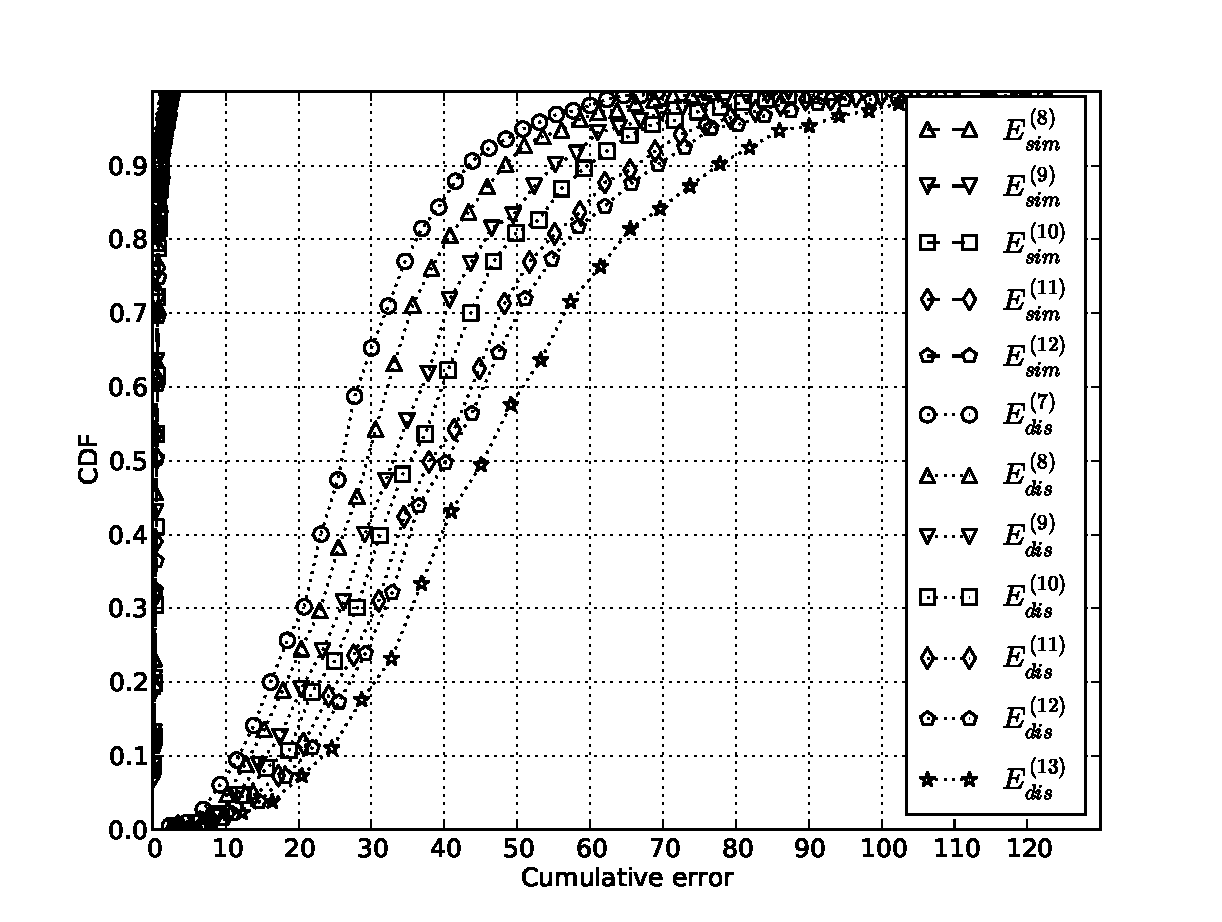
\includegraphics[width=1.1in, height=1in, viewport=0 15 530 400, clip]{everything_cdfs}
\label{subfigure:CDFs:Everything}}
\subfigure[Rates: Different Resolutions]	                    {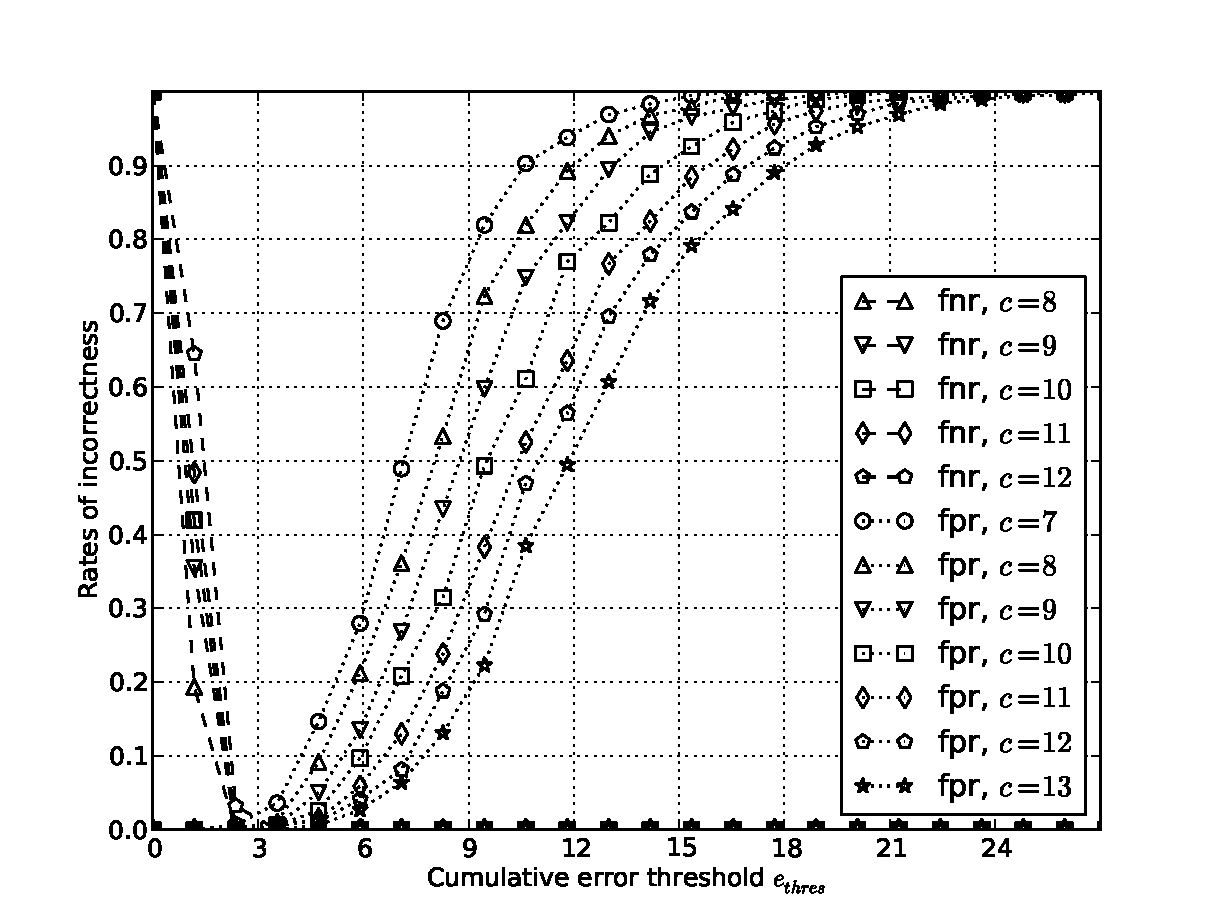
\includegraphics[width=1.1in, height=1in, viewport=0 15 530 400, clip]{resolutions_rates}
\label{subfigure:Rates:Different Resolutions}}
\subfigure[Rates: Watermarking (logo is $\frac{1}{4}$ width)]{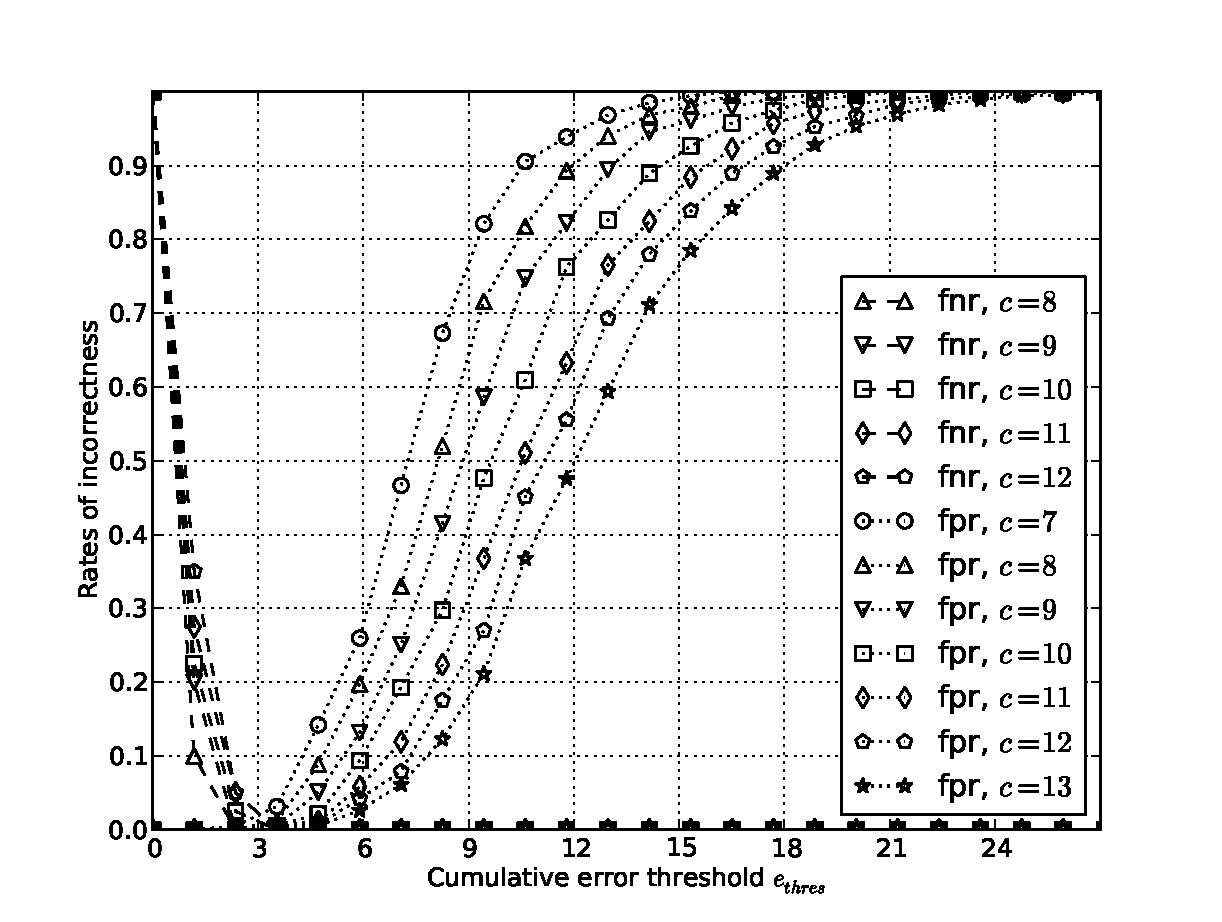
\includegraphics[width=1.1in, height=1in, viewport=0 15 530 400, clip]{watermarking4_rates}
\label{subfigure:Rates:Watermarking}} 
\subfigure[Rates: Everything]                                {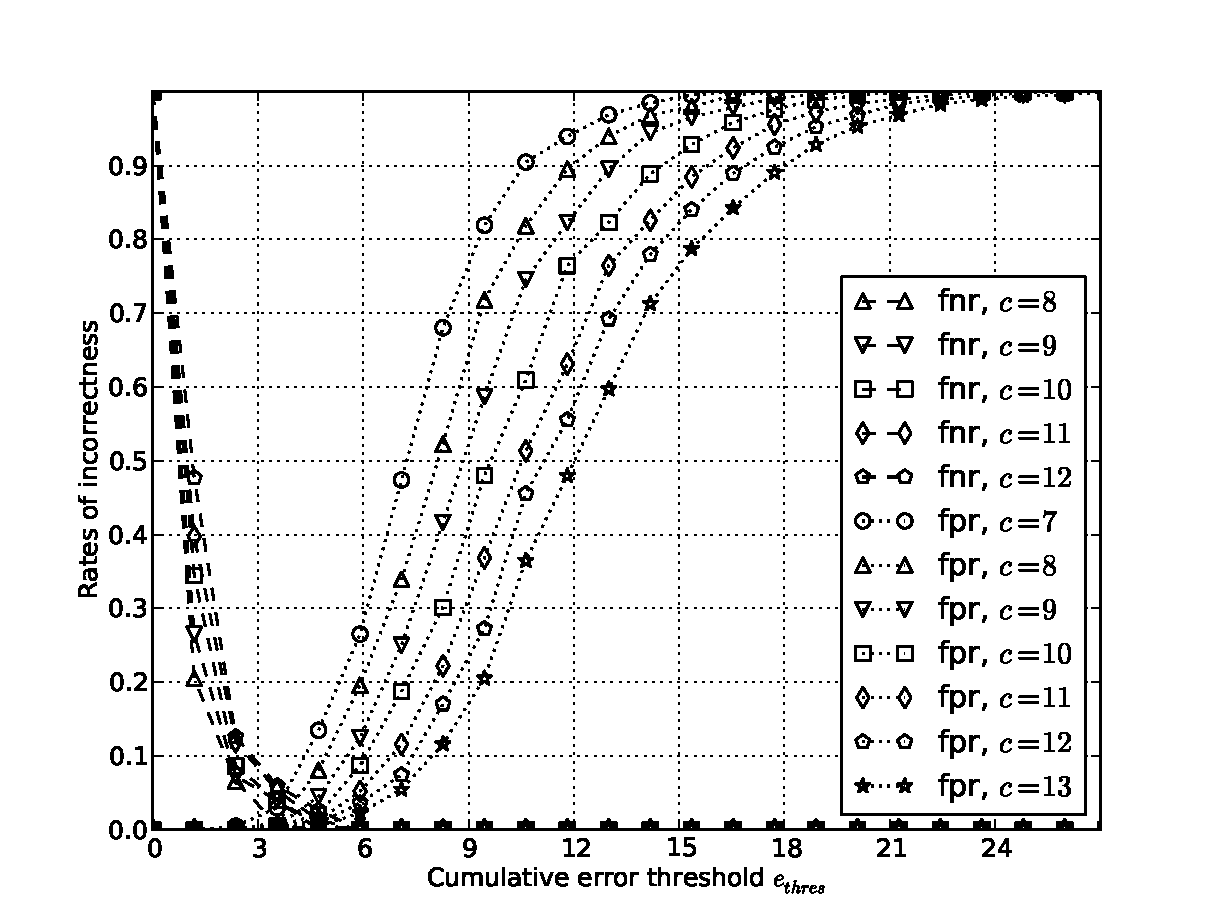
\includegraphics[width=1.1in, height=1in, viewport=0 15 530 400, clip]{everything_rates}
\label{subfigure:Rates:Everything}}

\caption{CDFs of Cumulative Errors and Rates of Incorrectness}
\label{figure:CDFs and Rates}
\end{figure*}

\subsection{Experiment 2: Filtering}
This experiment is similar to the first. We take the $20$ $360$p videos as our reference videos. For each $360$p video, we use FFmpeg to generate a sharpened version\footnote{Sharpening: ffmpeg -i in.flv -vf unsharp=13:13:5:13:13:5 out.flv} (using a spatial high pass filter), and also a blurred version\footnote{Blurring: ffmpeg -i in.flv -vf unsharp=13:13:-2:13:13:-2 out.flv} (using a low pass filter). This is shown for a single frame in one of our $20$ videos in Figs. \ref{subfigure:original}, \ref{subfigure:sharpened}, and \ref{subfigure:blurred}. These two filtered versions are the similar (human perception-wise) versions of the original $360$p video. All other videos are dissimilar. We repeat the experiment of comparing similar and dissimilar videos, as in the first experiment. The resulting CDFs and rates of incorrectness plots are very similar to Figs. \ref{subfigure:CDFs:Different Resolutions} and \ref{subfigure:Rates:Different Resolutions}, respectively. We omit them therefore, in the interest of space. As before, we can make a perfect similarity decision after $30$ seconds, given this data set.

\subsection{Experiment 3: Watermarking}
This experiment is again similar to the first. We take the $20$ $360$p videos as our reference videos. For each $360$p video, we use FFmpeg to generate two similar versions, each with an embedded logo.\footnote{Watermarking: ffmpeg -i in.flv -vf ``movie=logo.png, scale=logo\_width:logo\_height [wm]; [in][wm] overlay=logo\_x:logo\_y [out]'' out.flv} In the first, the logo is in the top left portion of the original video. In the second, the logo is in the bottom right portion. We consider two cases. In the first, the logo is a third of the original video's width. In the second, the logo is a quarter of the original video's width. This is shown for the second case in a single frame in one of our $20$ videos in Figs. \ref{subfigure:original}, \ref{subfigure:logo_tl}, and \ref{subfigure:logo_br}. The CDFs of the cumulative errors and the rates of incorrectness are shown in Figs. \ref{subfigure:CDFs:Watermarking} and \ref{subfigure:Rates:Watermarking}, respectively. The plots are similar as before. And as before, we can make a perfect similarity decision after $30$ seconds, given this data set.

\subsection{Experiment 4: Everything}
In this experiment, we combine all the possibilities of the previous three experiments. That is, each original $360$p reference video has up to eight possible similar versions (two different resolutions, two filtered versions, and four watermarked versions). The CDFs of the cumulative errors and the rates of incorrectness are shown in Figs. \ref{subfigure:CDFs:Everything} and \ref{subfigure:Rates:Everything}, respectively. Again, the plots are similar. This total data set has watermarked videos where the embedded logo is a third of the video's width. This unlikely large logo size causes imperfect similarity decisions. However, the rates of incorrectness are still very low. After $30$ seconds, fnr $= 0.03974$ and fpr $=0.00492$, for $e_{thres} = 3.54375$. Or, fnr $= 0$ and fpr $= 0.04494$, for $e_{thres} = 4.72500$. After $33$ seconds, fnr $= 0.03974$ and fpr $=0.00492$, for $e_{thres} = 3.54375$ (no change from $30$ seconds.) Or, fnr $= 0.00662$ and fpr $=0.02062$, for $e_{thres} = 4.72500$.


\section{Real-world Implementation Considerations}
\label{section:Real-world Implementation Considerations}
Our experiments provide practical parameters to use in a real-world implementation. We can use a larger data set of videos to further fine tune the various settings. However, our results indicate that after $30$ seconds, we can make a decision for similarity.

Our scheme is extremely efficient. We directly extract DCT coefficients from the incoming video byte stream in real time. Furthermore, for every $T = 3$ seconds, we only produce $192$ values using very light computations (just averaging) from the incoming video to compare against existing video signatures. Despite this simple and efficient algorithm, we still achieve extremely low rates of incorrectness, even approaching zero.

As the number of videos increase in our cache, the similarity detection computational load increases. However, this increase is actually sublinear. That is, many of the candidates can be eliminated in the first stage of the algorithm, as mentioned in Section \ref{subsection:Real-time Similarity Detection Algorithm}. We can easily filter out candidates that have different time lengths, compared to the incoming video. Furthermore, we can use other metadata, such as video content genre, title, keywords, etc. to further filter out unlikely candidates. In fact, the entire first stage deals with content-aware video indexing, and is beyond the scope of this work. Therefore, even if a video is made up of multiple sections of other videos spliced together, this first stage should be able to avoid false positive similarity decisions.

\section{Conclusion}
\label{section:Conclusion}
We present an efficient real-time similarity detection system for video caching and streaming. Our scheme is computationally light, but still achieves rates of incorrectness approaching zero, after just $30$ seconds of downloading an incoming video.

For future work, we plan to investigate more modern codecs and container formats. In particular, we seek to efficiently extract information directly from the video byte stream that can serve as robust video signatures. In addition, we seek effective content-aware indexing schemes in order to filter out candidates prior to similarity detection. This is stage one in Section \ref{subsection:Real-time Similarity Detection Algorithm}.

\begin{thebibliography}{99}


\bibitem{Songqing Chen}
S. Chen, H. Wang, X. Zhang, B. Shen, and S. Wee, ``Segment-Based Proxy Caching for Internet Streaming Media Delivery," in \emph{IEEE MultiMedia}, vol. 12, no. 3, pp. 59-67, Jul.-Sep. 2005. 

\bibitem{Wei Tu}
W. Tu, E. Steinbach, and X.Li, ``Proxy Caching for Video-on-Demand Using Flexible Starting Point Selection," in \emph{IEEE Transactions on Multimedia}, vol. 11, no. 4, pp. 716-729, Jun. 2009.

\bibitem{Dohy Hong}
D. Hong, D. De Vleeschauwer, and F. Baccelli, ``A Chunk-based Caching Algorithm for Streaming Video," in \emph{Proc. Workshop on Network Control and Optimization (NETCOOP)}, Ghent, Belgium, Nov.-Dec. 2010, pp. 33-40.

\bibitem{Yago Sanchez}
Y. S\'anchez, T. Schierl, C. Hellge, T. Wiegand, D. Hong, D. De Vleeschauwer, W. Van Leekwijck, and Y. Lelouedec, ``Improved caching for HTTP-based Video on Demand using Scalable Video Coding," in \emph{Proc. IEEE Consumer Communications and Networking Conference (CCNC)}, Las Vegas, NV, Jan. 2010, pp. 595-599.

\bibitem{Jing Li}
J. Li, J. Yang, and H. Xi, ``A Scalable and Cooperative Caching Scheme in a Distributed VOD System," in \emph{Proc. IEEE International Conference on Communication Software and Networks (ICCSN)}, Macau, China, Feb. 2009, pp. 247-250.

\bibitem{Byoung-Jip Kim}
B.-J. Kim, K. Kim, and D. Park, ``The Content-Aware Caching for Cooperative Transcoding Proxies," in \emph{Proc. International Conference on Information Networking, Convergence in Broadband, and Mobile Networking (ICOIN)}, Jeju Island, Korea, Jan.-Feb. 2005, pp. 766-775.

\bibitem{Chuanyi Liu}
C. Liu, Y. Lu, C. Shi, G. Lu, D.H.C. Du, D.-S. Wang, ``ADMAD: Application-Driven Metadata Aware De-duplication Archival Storage System," in \emph{Proc. IEEE International Workshop on Storage Network Architecture and Parallel I/Os (SNAPI)}, Baltimore, MD, Sep. 2008, pp. 29-35.

\bibitem{Atul Katiyar}
A. Katiyar and J.B. Weissman, ``ViDeDup: An Application-Aware Framework for Video De-duplication," in \emph{Proc. USENIX Workshop on Hot Topics in Storage and File Systems (HotStorage)}, Portland, OR, Jun. 2011.

\bibitem{Sen-ching S. Cheung}
S.S. Cheung and A. Zakhor, ``Efficient Video Similarity Measurement with Video Signature," in \emph{IEEE Transactions on Circuits and Systems for Video Technology}, vol. 13, no. 1, pp. 59-74, Jan. 2003.

\bibitem{Xian-Sheng Hua}
X.-S. Hua, X. Chen, and H.-J. Zhang, ``Robust Video Signature based on Ordinal Measure," in \emph{Proc. IEEE International Conference on Image Processing (ICIP)}, Singapore, Oct. 2004, vol.1, pp. 685-688.

\bibitem{web:SWF}
``SWF File Format Specification Version 10," \emph{Adobe Systems Incorporated}.

\bibitem{web:H.263}
``Video coding for low bit rate communication, Recommendation H.263," \emph{International Telecommunication Union}.

\bibitem{web:FFmpeg}
``FFmpeg." [Online]. Available: http://ffmpeg.org.

\end{thebibliography}

%In LaTeX, to start a new column (but not a new page) and help balance the
%last-page column lengths, you can use the command ``$\backslash$pagebreak'' as
%demonstrated on this page (see the LaTeX source below).

% To start a new column (but not a new page) and help balance the last-page
% column length use \vfill\pagebreak.
% -------------------------------------------------------------------------
%\vfill
%\pagebreak



\end{document}
